Mit Hilfe des zuvor in Kapitel \ref{ch:Grundlagen} erworbenen Wissens stellen wir in diesem Kapitel einen temporalen 
Algorithmus, basierend auf der Arbeit von \cite{hal02158423}, vor. Dieser erreicht eine zeitlich stabile 
\nameref{ch:Content1:sec:blue noise} Fehlerverteilung innerhalb weniger Bilder im Bildraum. Dabei wird in 
dieser Arbeit im Speziellen auf den Einsatz innerhalb Echtzeitanwendungen eingegangen. 
Der Algorithmus arbeitet mit drei separaten Schritten: 
In einem ersten Schritt sortiert \ref{ch:Content2:sec:Sorting} der Algorithmus anhand unser getroffenen 
\nameref{ch:Content2:sec:a Posteriori} Annahmen die Anfangswerte unseres \nameref{ch:Content1:sec:Path Tracer}
derart um, sodass die im nächsten Bilderzeugungsschritt entstehenden Pixel \nameref{ch:Content1:sec:blue noise}
verteilt sind. Die Notwendigkeit des nächsten Schrittes, das \nameref{ch:Content2:sec:Retargeting}, ergibt sich 
aus der Tatsache, dass wir in jedem Bilderzeugungsschritt eine neue blue noise Textur verwenden (theoretisch,
praktisch benutzen wir \nameref{ch:Content1:sec:Quasi-Zufallsfolgen}). Ohne die angewandte Permutation innerhalb 
des Schrittes würde sich durch die Randomisierung die jeweilige gewonnene blue noise Verteilung nicht auf den 
nächsten Bilderzeugungsprozess übertragen.  
Der Algorithmus, bestehend aus zwei grundsätzlichen Schritten, das Umsortieren und Permutieren, 
verlangt folgende Vorbedingung:
benachbarte Pixel müssen annähernd den selben Wert haben (siehe Abschnitt \ref{ch:Content1:sec:blue noise sampling}
und Abschnitt \ref{subsec:Praktische_Durchführung}). Da wir einen temporalen Algorithmus haben, soll diese Annahme 
auch über mehrere gerenderte Bilder hinweg gelten. Es sollte also beachtet werden, dass der Algorithmus z.B. nicht 
für Objektkanten oder ruckartige Bewegungen (der Kamera oder Objekte) ausgelegt ist.
Aufgrund dieses Problems nehmen wir eine Idee zur Verbesserung des Algorithmus auf (siehe \cite{hal02158423}) und führen 
damit einen neuen temporalen Projektionsschritt in Abschnitt \ref{alg:TemporalAccumulation} ein. Damit wird sich die 
zeitliche Stabilität erhöhen.
 

\begin{figure}[H]
    \begin{subfigure}{\textwidth}
        \centering 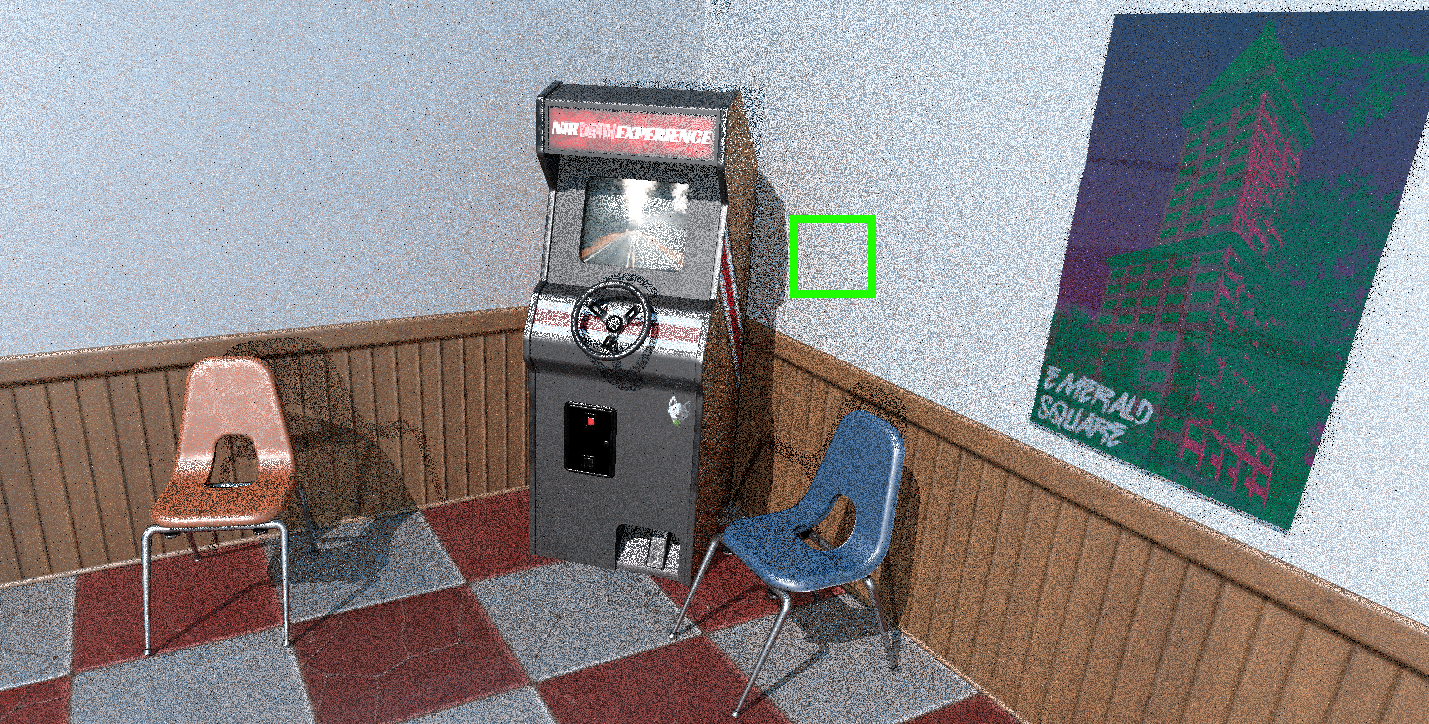
\includegraphics[width=0.7\linewidth]{content/TemporalerAlg/Bilder/WhiteNoise/Szene.png}
        \caption{Szene}
        \label{fig:Szene_Weißes Rauschen}
    \end{subfigure}
    \begin{subfigure}{0.5\textwidth}
        \centering 
\includegraphics[width=0.5\linewidth]{content/TemporalerAlg/Bilder/WhiteNoise/Ausschnitt.png} 
        \caption{Szenenausschnitt}
        \label{fig:ausschnitt_Weißes_Rauschen}
    \end{subfigure}
    \begin{subfigure}{0.5\textwidth}
        \centering 
\includegraphics[width=0.5\linewidth]{content/TemporalerAlg/Bilder/WhiteNoise/Spektrum.png}
        \caption{Fouriertransformierte des Ausschnitts}
        \label{fig:Fouriertransformierte_Weißes_Rauschen}
    \end{subfigure}
        \caption{Ausgangssituation, erstes erzeugte Bild}
        \label{fig:Path Tracer mit zufälligen Seeds}
\end{figure}

In Abbildung \ref{fig:Path Tracer mit zufälligen Seeds} sehen wir die erste Ausgabe des \nameref{ch:Content1:sec:Path Tracer}
aufgrund zufälliger Anfangswerte (erzeugt mit Mersenne-Twister). Dies ist der Startzustand für unseren Algorithmus.
Wie bereits in Abschnitt \ref{ch:Content1:sec:blue noise} ausführlich besprochen, lassen sich anhand der Szene, des Szenenausschnitts 
und dem korrespondierenden Spektrum die typischen Eigenschaften einer white noise ablesen (Clusterbildung im Zeitbereich, 
gleichmäßige Amplitudendichte im Frequenzbereich).
Nehmen wir diese Ausgabe des Path Tracers, so lassen sich mit den erzeugten Pixeln nachträgliche Annahmen (siehe Abschnitt \ref{ch:Content2:sec:a Posteriori})
für ihn formulieren.
